% ----- formatovani dokumentu -----------------------------------------------
\documentclass[12pt,a4paper,titlepage,final]{report}
\usepackage[utf8]{inputenc}
\usepackage[T1, IL2]{fontenc}
\usepackage{graphicx}
\usepackage{epstopdf}
\usepackage[margin=2cm]{caption}
\usepackage[top=3cm, left=2cm, right=2cm, text={17cm, 24cm}, ignorefoot]{geometry}
\usepackage{color}
\usepackage{url}
\usepackage{setspace}
\singlespacing
\usepackage[square, numbers]{natbib} 
\pagestyle{plain}
\pagenumbering{arabic}
\setcounter{page}{1}
\setcounter{secnumdepth}{-1}
\setlength{\parindent}{1cm}	
\usepackage{natbib}
\usepackage{float}

% ----- vyberte jazyk -------------------------------------------------------
\usepackage[english,czech]{babel}
%\usepackage[english]{babel}

% ----- dopiste titulky -----------------------------------------------------
\newcommand\Course{Počítačová grafika}
\newcommand\WorkTitle{Šachy pomocí ray-tracing}
\newcommand\AuthorA{Ivan Ševčík}
\newcommand\AuthorAEmail{xsevci50@stud.fit.vutbr.cz}
\newcommand\AuthorB{Adam Jež}
\newcommand\AuthorBEmail{xjezad00@stud.fit.vutbr.cz}
\newcommand\AuthorC{Tomáš Mlynarič}
\newcommand\AuthorCEmail{xmlyna06@stud.fit.vutbr.cz}
\newcommand\Faculty{Fakulta Informačních Technologií}
\newcommand\School{Vysoké Učení Technické v Brně}

\usepackage[
pdftitle={\WorkTitle},
pdfauthor={\AuthorA, \AuthorB, \AuthorC},
bookmarks=true,
colorlinks=true,
breaklinks=true,
urlcolor=blue,
citecolor=blue,
linkcolor=blue,
unicode=true,
]
{hyperref}


% ----- titulni strana ------------------------------------------------------

\begin{document}
	\begin{titlepage}
	\begin{center}
		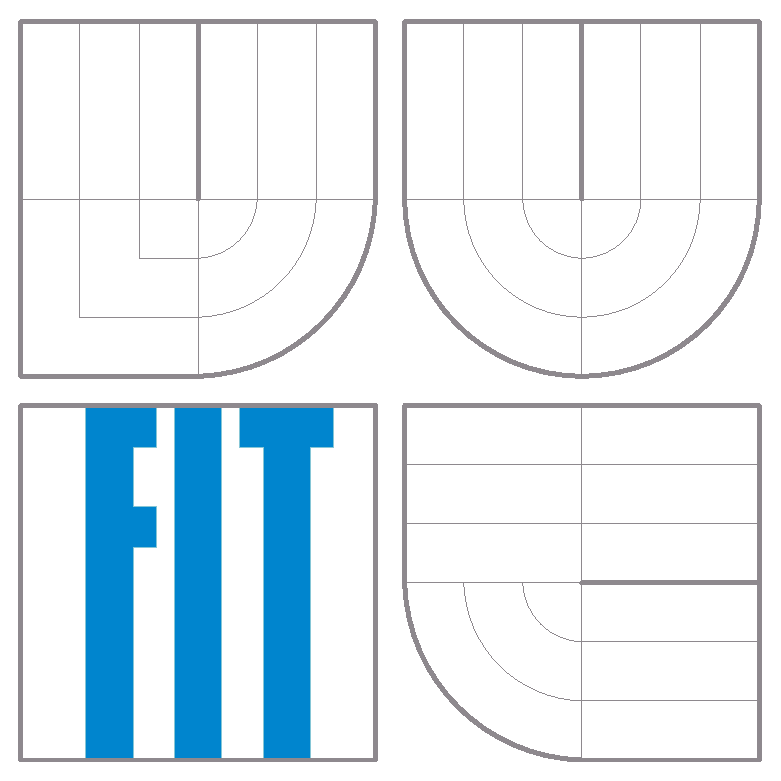
\includegraphics[height=5cm]{images/logo.eps}
	\end{center}
	\vfill
	\begin{center}
		\begin{Large}
			\Course\\
		\end{Large}
		\bigskip
		\begin{Huge}
			\WorkTitle\\
		\end{Huge}
	\end{center}
	\vfill
	\begin{center}
		\begin{large}
			\today
		\end{large}
	\end{center}
	\vfill
	\begin{flushleft}
		\begin{large}
			\begin{tabular}{lll}
				Autoři: & \AuthorA, & \url{\AuthorAEmail} \\
				        & \AuthorB, & \url{\AuthorBEmail} \\
				        & \AuthorC, & \url{\AuthorCEmail} \\
				& & \\
				& \Faculty \\
				& \School \\
			\end{tabular}
		\end{large}
	\end{flushleft}
\end{titlepage}		
	
% ----- obsah --------------------------------------------------------------
	
\tableofcontents

% ----- zadani -------------------------------------------------------------
\newpage
\chapter{Zadání}

Úlohou bylo implementovat libovolný typ ray-traceru a s jeho pomocí vizualizovat scénu složenou ze šachovnice a šachových figurek. Důraz měl být kladen na jevy, které se jen obtížne vizualizují pomocí klasických vykreslovacích technik a na kvalitu výsledného zobrazení. Z těchto jevů jsme si tedy zvolily stíny a odlesky. Navíc je nutné implementovat uložení stavu šachovnice, která by byla vhodná pro interakci se šachovým strojem nebo uživatelem přes GUI. Důležitá je také parametrizovatelnost procesu vykreslování.

Vzhledem na účel by bylo žádoucí také aby překreslování bylo plynulé, proto se také zaměříme na optimalizace a další techniky urychlení výpočtu. Dále by bylo určitě pro uživatele pohodlné mít možnost zachytiť snímek a uložit ho do souboru bez nutnosti dělat printscreen a ořezávání, a také mít možnost uložit rozehranou partii a později v ní pokračovat.   

Celkově je tedy nutné věnovat se v rámci projektu těmto částem:
\begin{itemize}
	\item Raytracer
	\begin{itemize}
		\item Odlesky a stíny
		\item Antialiasing
		\item Parametrizovatelnost
		\begin{itemize}
			\item Změna pohledu kamery
			\item Změna pozice světla
			\item Stupeň antialiasingu
			\item Počet odlesků
		\end{itemize}
	\end{itemize}
	\item Šachová partie
	\begin{itemize}
		\item Vhodná reprezentace
		\item Možnost uložení do souboru
		\item Možnost uložit snímek 
	\end{itemize}
	\item Plynulost překreslování
	\begin{itemize}
		\item Profilování a optimalizace kritických částí
		\item Paralelizace výpočtu
	\end{itemize}
\end{itemize}

\chapter{Použité technologie}
Program je napsán v jazyku \texttt{c\#} pro \texttt{.Net 4.5} a kromě knižnice OpenTK nevyžaduje ke svému běhu nic jiného. Použité uživatelské rozhraní je už poměrne staré ale pro naše účely postačující \texttt{WinForms} z důvody přenositelnosti.

Při vývoji bylo použito \texttt{Visual Studio} a verzovací systém \texttt{git} s repozitářem na službě \texttt{GitHub}. Vyvíjelo se pod operačními systémy \texttt{Windows} a \texttt{OS X} a testování výsledného programu proběhlo také na systému \texttt{Linux}, konkrétně distribuce \texttt{Lubuntu}, kde bylo pro skompilování použito \texttt{MonoDevelop}.


\begingroup
\let\clearpage\relax
\chapter{Použité zdroje}
Při tvorbě projektu jsme si propůjčili značnou část ray-traceru Aurelius dostupného ze stránek předmětu PGR \cite{aurelius}, který sme však dále rozširovali, například implementováním konečného válce a kuželu. Oběcný kužel byl implementován pomocí rovnic uvedených v přednášce ze zahraniční univerzity \cite{cone}. Dále rovnici pro reflekci sme našli na webu \cite{reflect} a phongov osvětlovací model byl ozřejmen také pomocí webu \cite{phong}. Efektivní test průniku paprsku s obalovacím kvádrem sme našli na stránce \cite{aabb}.

\endgroup

%---------------------------------------------------------------------------
\chapter{Nejdůležitější dosažené výsledky}

\section{Krása výsledku}

Spojením textur, phongovho stínovacího modelu, odlesků, odrazů, stínů a antialiasingu se podařilo dosáhnout vizuálně velice pěkného výsledku při vykreslování. Dále byly vytvořeny nevšední modely figurek, pro které byli následně přirazeny farby a další parametry tak, aby scénu udělali co nejzajímavější. Dále už jen uvádíme několik obrázků, které výsledek demonstrují nejlépe.

\begin{center}
	\captionsetup{type=figure}
		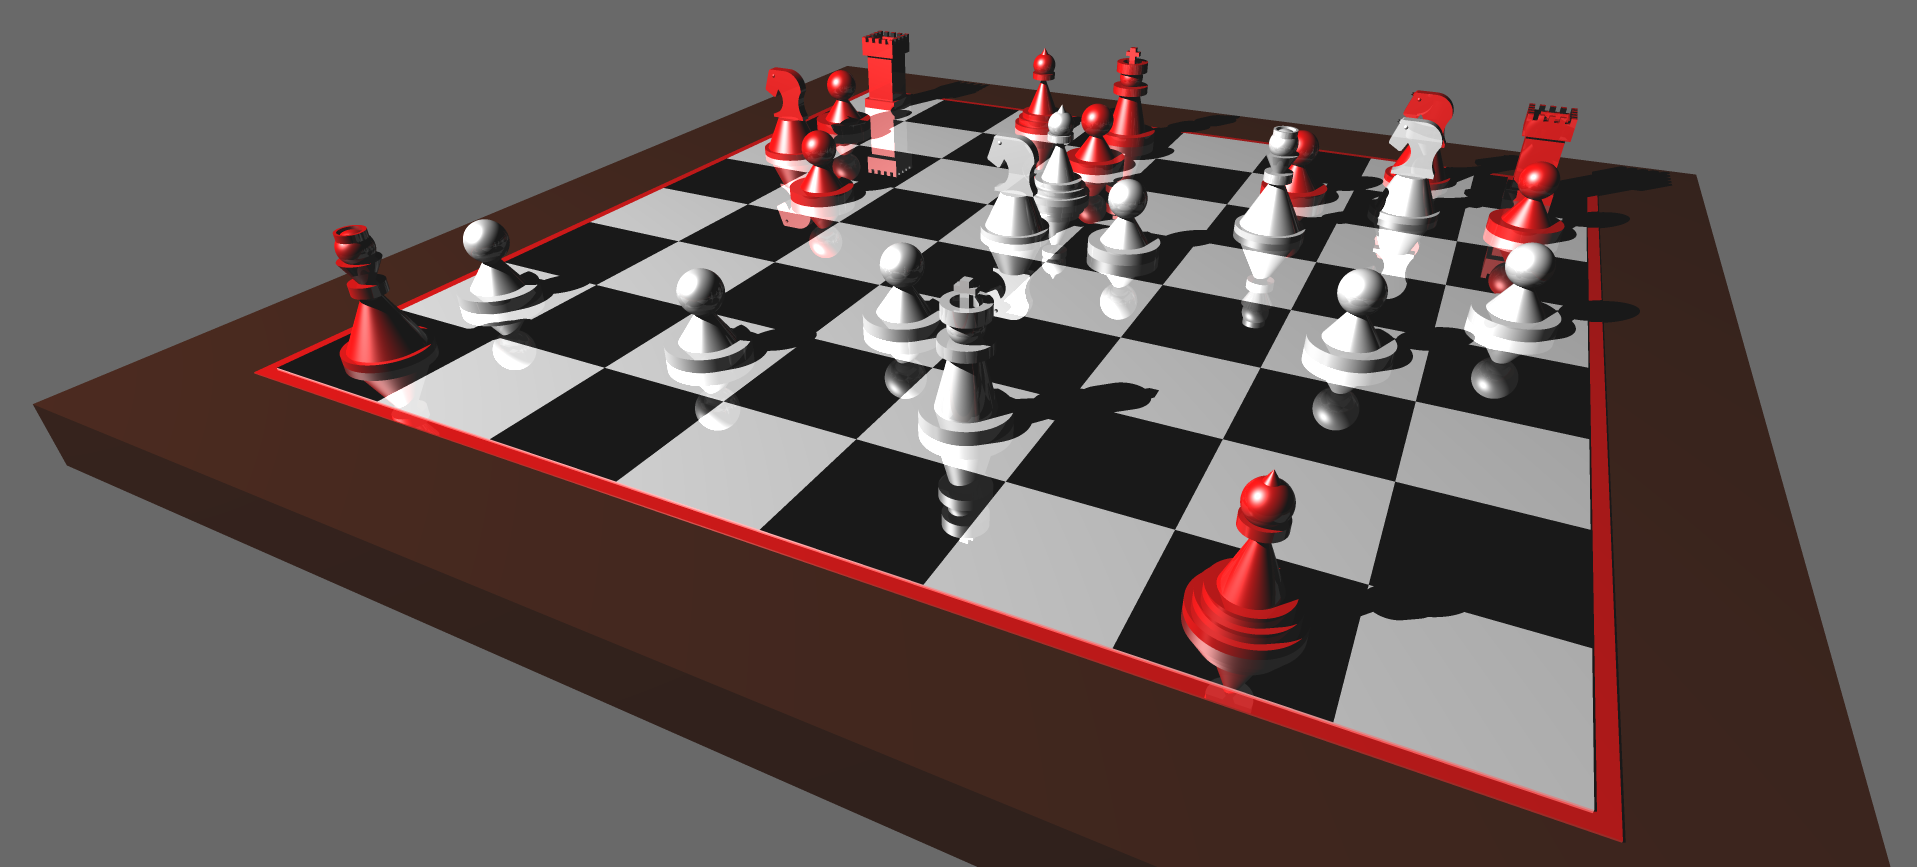
\includegraphics[width=0.8\linewidth]{images/scene1.png}
	\captionof{figure}{Základní vizualizace libovolné partie}
\end{center}

\begin{center}
	\captionsetup{type=figure}
	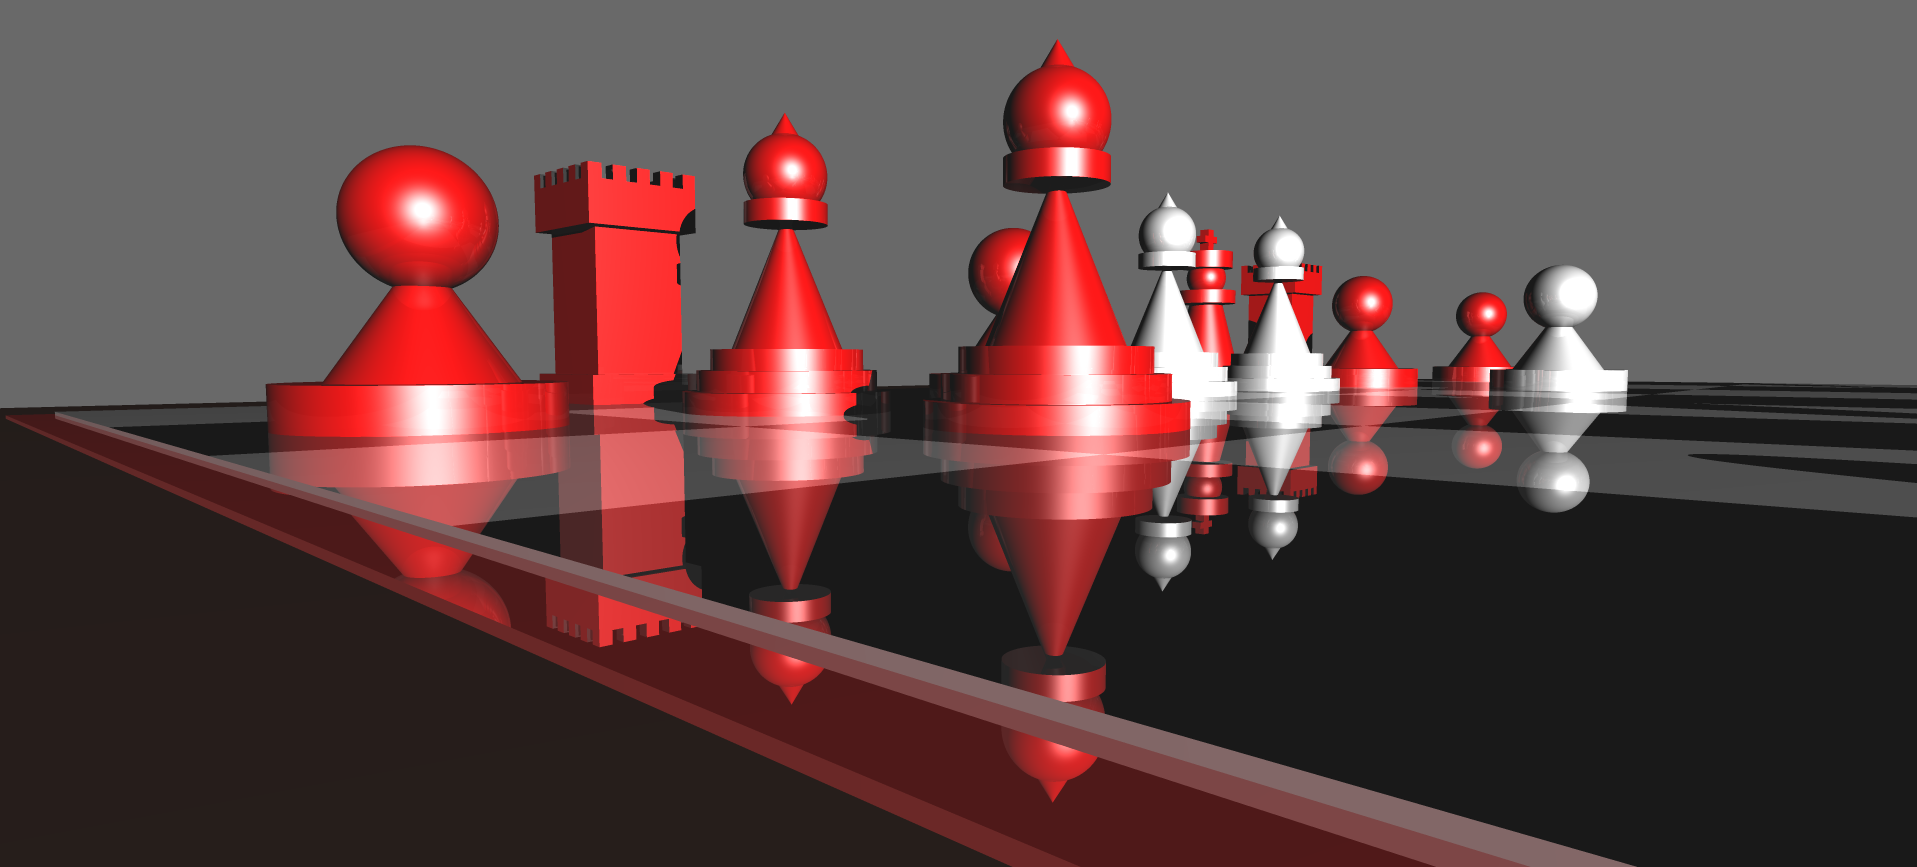
\includegraphics[width=0.8\linewidth]{images/scene2.png}
	\captionof{figure}{Různá míra reflekce materiálu}
\end{center}

\begin{center}
	\captionsetup{type=figure}
	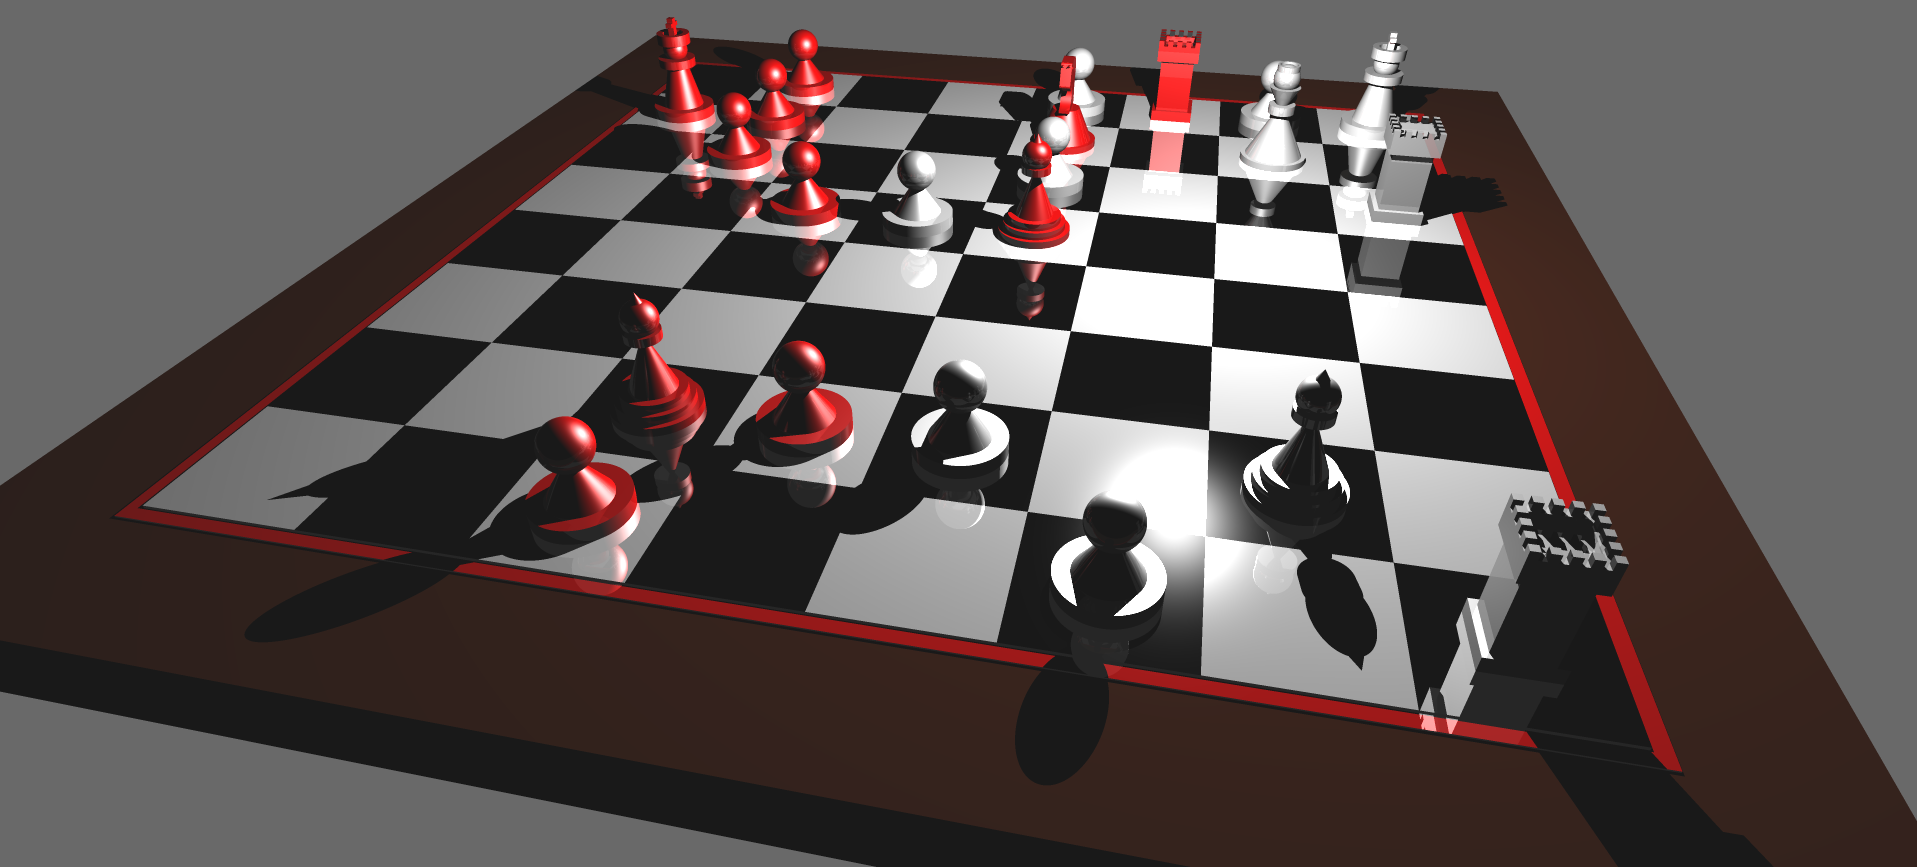
\includegraphics[width=0.8\linewidth]{images/scene3.png}
	\captionof{figure}{Stínování a vrhaní stínů}
\end{center}

\section{Příjemná manipulace}
Se scénou je možné jednoduše manipulovat jen pomocí myši a toto ovládaní je intuitivní. Kamerou je možné kroužit kolem bodu ve scéně, přibližovat nebo oddalovat, a také pohybovat ve směru osí kamery. Kombinace rotace a posunu podél osí kamery umožňuje přesun na libovolnou pozici v 3D prostor, i když pohyb myší po obrazovce poskytuje jen 2D souřadnice. Dále je možné pomocí myši jednoduše měniť pozici světla a tedy interaktívne vizualizovat různé stíny a odlesky.

\section{Dosáhnoutá překreslovací frekvence}

Náš první pokus s ray-tracingem využíval hraniční reprezentaci pomocí trojuholníků. Čas vytvoření jednoho snímku pro jeden model konvice bez jakýchkoliv efektů a jen s plochým stínováním se pohyboval kolem 40-ti sekund. To bylo neúnosné z hlediska přidávání další funkcionality, proto sme se rozhodli přejít na CSG reprezentaci, která sama o sobě urychlila výpočet přibližne stonásobně, ovšem pro jiný ale podobně složitý model. Dále jsme zavedli obalovací tělesa, konkrétně AABB (Axis-aligned bounding box), které opět významně urychlili výpočet odstraněním značného počtu testů vůči poměrne komplikované CSG geoetrii. Také byla zavedena paralelizace výpočtu na CPU pomocí vláken, která ale neměla už tak výrazný vplyv na zrychlení.

Pro plynulou interakci s uživatelem však byl zaveden \textit{odlehčený} vykreslovací mód jak je možné vidět na obrázku \ref{camera}, který se zapne při pohybu kamerou. Po zapnutí se pak vykreslují pouze stínovaná obalovací tělesa, které pro uživatele obvykle stačí pro představu kde v scéně se kamera nachází, no vykreslování je mnohem rychlejší. Kde to bylo možné se využívá cache objektů, například v případe, že se neměnila pozice kamery je možné znovu využít stejných paprsků jak při posledním vykreslování, a také některé mezivýsledky z různych výpočtů bylo možné uložit pro další použití.

\begin{figure}[H]
	\centering
	\captionsetup{type=figure}
	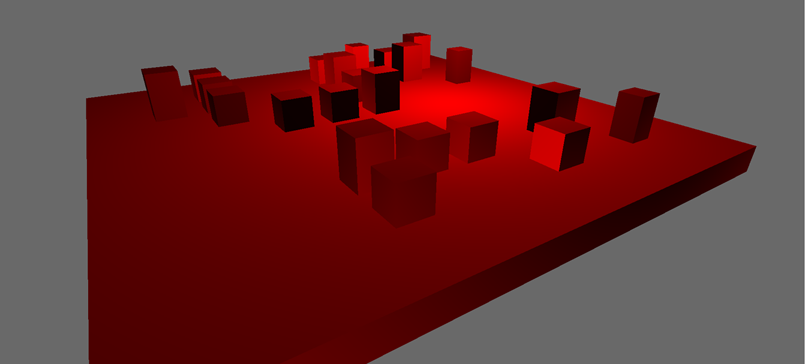
\includegraphics[width=0.8\linewidth]{images/camera.png}
	\captionof{figure}{Vykreslování počas pohybu kamerou}
	\label{camera}
\end{figure}

Výsledkem je vzhledem na metodu vykreslování vcelku uspokojivá překreslovací frekvence při rozumném rozlíšení. Nasledujíci tabulka dáva lepší představu o těchto hodnotách.

\begin{table}[H]
	\begin{center}
		\begin{tabular}{| l | c | c | c | c| c | c |}
			\hline
			Rozlíšení & 600x400 & 600x400 & 600x400 & 600x400 & 600x400 & 1917x867
			\\ \hline
			
			Počet vláken & 1 & 8 & 8 & 8 & 8 & 8
			\\ \hline
			
			Počet reflekcí & 0 & 0 & 2 & 2 & 2 & 2
			\\ \hline
			
			Antialiasing & 1 & 1 & 1 & 1 & 2 & 1
			\\ \hline
			
			Kamera v pohybu & Ne & Ne & Ne & Áno & Ne & Ne
			\\ \hline
			
			\textbf{FPS} & 0.81 & 2,6 & 1,42 & 5,8 & 0,34 & 0,23
			\\ \hline
		\end{tabular}
	\end{center}	
	\caption{Překreslovací frekvence pro různe konfigurace}  
\end{table}

%---------------------------------------------------------------------------
\chapter{Práce na projektu}

\section{Rozdělení práce v týmu}
Pokud to bude vhodné, použijte odrážky místo souvislých vět.

\paragraph{Rozsah:} co nejstručnější tak, aby bylo zřejmé, jak byla dělena práce a za co v
projektu je kdo zodpovědný.

\begin{itemize}
\item \textbf{\AuthorA}: Udělal todle, tamto, vlastně skoro všechno
\item \textbf{\AuthorB}: Neudělal skoro nic, ale dělal zbytku týmu kafe
\end{itemize}

%---------------------------------------------------------------------------
\section{Co bylo nejpracnější}

Popište, co vám při řešení nejvíce komplikovalo život, s čím jste se museli
potýkat, co zabralo čas.

\paragraph{Rozsah:} 5-10 řádků

\begin{itemize}
\item \textbf{\AuthorA}: Prácné bylo todle a tamto.
\item \textbf{\AuthorB}: Pracné bylo vyvážit poměr kafe, mléka a cukru. 
\end{itemize}


%---------------------------------------------------------------------------
\section{Zkušenosti získané řešením projektu}

Popište, co jste se řešením projektu naučili. Zahrňte dovednosti obecně
programátorské, věci z oblasti počítačové grafiky, ale i spolupráci v týmu,
hospodaření s časem, atd.

\paragraph{Rozsah:} formulujte stručně, uchopte cca 3-5 věcí

%---------------------------------------------------------------------------
\chapter{Autoevaluace}

Ohodnoťte vaše řešení v jednotlivých kategoriích (0 – nic neuděláno,
zoufalství, 100\% – dokonalost sama). Projekt, který ve finále obdrží plný
počet bodů, může mít složky hodnocené i hodně nízko. Uvedení hodnot blízkých
100\% ve všech nebo mnoha kategoriích může ukazovat na nepochopení problematiky nebo na snahu kamuflovat slabé stránky projektu. Bodově hodnocena bude i
schopnost vnímat silné a slabé stránky svého řešení.

\paragraph{Technický návrh (50\%):} (analýza, dekompozice problému, volba
vhodných prostředků, $\ldots$) 
Stručně (1-2 řádky) komentujte hodnocení. 

\paragraph{Programování (50\%):} (kvalita a čitelnost kódu, spolehlivost běhu,
obecnost řešení, znovupoužitelnost, $\ldots$)
Stručně (1-2 řádky) komentujte hodnocení. 

\paragraph{Vzhled vytvořeného řešení (50\%):} (uvěřitelnost zobrazení,
estetická kvalita, vhled GUI, $\ldots$)
Stručně (1-2 řádky) komentujte hodnocení. 

\paragraph{Využití zdrojů (50\%):} (využití existujícího kódu a dat, využití
literatury, $\ldots$)
Stručně (1-2 řádky) komentujte hodnocení. 

\paragraph{Hospodaření s časem (50\%):} (rovnoměrné dotažení částí projektu,
míra spěchu, chybějící části řešení, $\ldots$)
Stručně (1-2 řádky) komentujte hodnocení. 

\paragraph{Spolupráce v týmu (50\%):} (komunikace, dodržování dohod, vzájemné
spolehnutí, rovnoměrnost, $\ldots$)
Stručně (1-2 řádky) komentujte hodnocení. 

\paragraph{Celkový dojem (50\%):} (pracnost, získané dovednosti, užitečnost,
volba zadání, cokoliv, $\ldots$)
Stručně (5-10 řádků) komentujte hodnocení. 

%---------------------------------------------------------------------------
\chapter{Ovládání vytvořeného programu}
Stručně popište, jak se program ovládá (nejlépe odrážky rozdělené do
kategorií). Pokud se ovládání odchyluje od zkratek a způsobů obvykle
používaných v okýnkových nadstavbách operačních systémů, zdůvodněte, proč se
tak děje.

\paragraph{Rozsah:} odrážky nebo jednoduchý popis a odrážky


%---------------------------------------------------------------------------
\chapter{Doporučení pro budoucí zadávání projektů}

Co vám vyhovovalo a co nevyhovovalo na organizaci projektů? Které prvky by měly být zachovány, zesíleny, potlačeny, eliminovány?

%---------------------------------------------------------------------------

\chapter{Různé}

Ještě něco by v dokumentaci mělo být? Napište to sem! Podle potřeby i založte
novou kapitolu.

%---------------------------------------------------------------------------

\bibliographystyle{plain}

\nocite{cite1}
\nocite{cite2}
\nocite{cite3}

\bibliography{reference}
\addcontentsline{toc}{chapter}{Literatura}

\end{document}

